% flashcards-title: Ruler scale with two pointer arrows
% flashcards-desc: A horizontal measuring scale from zero to six with a longer labeled mark at every whole centimeter and ten equal small steps between neighboring labeled marks. Two arrows above the scale, labeled A and B, each point down at the scale: A at one of the labeled marks and B between two labeled marks.
\documentclass[tikz]{standalone}
\usetikzlibrary{arrows.meta,patterns}

\definecolor{qraNavy}{HTML}{17324D}
\definecolor{qraBlue}{HTML}{2B6CB0}
\definecolor{qraGold}{HTML}{B7791F}
\definecolor{qraPale}{HTML}{EAF2F8}
\definecolor{qraGray}{HTML}{5C6773}

\tikzset{
  qra axis/.style={draw=qraNavy, line width=1.2pt},
  qra tick/.style={draw=qraNavy, line width=1pt},
  qra guide/.style={draw=qraGray, densely dashed, line width=0.8pt},
  qra counter/.style={circle, draw=qraNavy, fill=qraPale, line width=0.9pt, minimum size=7mm, inner sep=0pt},
  qra label/.style={font=\sffamily\bfseries, text=qraNavy},
  qra small label/.style={font=\sffamily, text=qraNavy},
}

\begin{document}
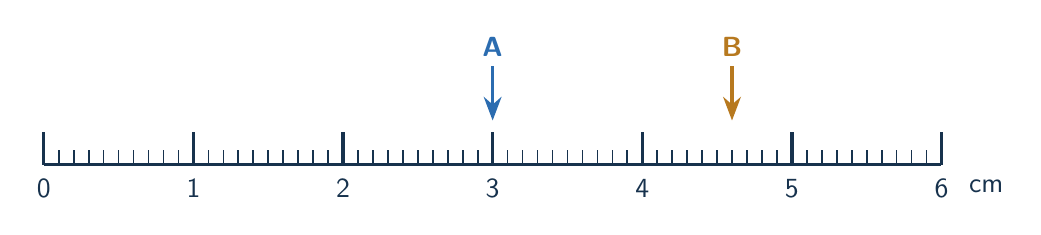
\begin{tikzpicture}[x=1.9cm,y=1cm]
  % baseline
  \draw[qra axis] (0,0) -- (6,0);
  % minor ticks at tenths
  \foreach \i in {0,...,60}
    \draw[qra tick, line width=0.6pt] (\i*0.1,0) -- (\i*0.1,0.18);
  % major ticks and labels
  \foreach \x in {0,...,6} {
    \draw[qra tick, line width=1.2pt] (\x,0) -- (\x,0.42);
    \node[qra small label, below] at (\x,-0.06) {\x};
  }
  \node[qra small label, anchor=west] at (6.12,-0.28) {cm};
  % pointer arrows with letter labels (redundant non-color cue)
  \draw[draw=qraBlue, line width=1.2pt, -{Stealth[length=3mm]}] (3,1.25) -- (3,0.56);
  \node[qra label, text=qraBlue] at (3,1.5) {A};
  \draw[draw=qraGold, line width=1.2pt, -{Stealth[length=3mm]}] (4.6,1.25) -- (4.6,0.56);
  \node[qra label, text=qraGold] at (4.6,1.5) {B};
\end{tikzpicture}
\end{document}
